\documentclass{article}

\usepackage{lmodern}
\usepackage[UTF8]{ctex}% 中文语言包
\usepackage{amsmath}
\usepackage{booktabs}% 引入三线表宏包
\usepackage{indentfirst}% 使用indentfirst宏包
\setlength{\parindent}{2em}% 设置首行缩进距离
\usepackage{graphicx}% 插入图片宏包
\usepackage{float}% 图片错位解决

\title{微机原理}

\author{XDwan}

\begin{document}
    
\renewcommand{\contentsname}{目录}%将content转为目录
\tableofcontents
\newpage

\section{绪论}

\section{单核处理器8086/8088}

单核处理器是多核处理器的基础

从8086开始 Intel CPU设计采用了向后兼容,也称向下兼容

单核的8086 CPU 成为其后Intel CPU的基石

\subsection{8086/8088处理器功能特性}

\begin{enumerate}
    \item 第一次将流水线思想引进微处理器:指令级流水
    \item 存储器分段管理机制引入处理器,扩大寻址能力
    \item 只有整数运算指令。配套数值协处理器8087、输入输出协处理器8089,具备较强大的计算能力和I/O处理能力
\end{enumerate}

8086 CPU有三个版本 8086、8086-2、8086-1。仅时钟频率不同,依次为5Mhz、8Mhz、10Mhz。
具有以下功能特性:

\begin{enumerate}
    \item 直接主存寻址能力1MB
    \item 体系结构针对强大的汇编语言和有效的高级语言设计
    \item 14个16位寄存器
    \item 24种操作数寻址方式
    \item 操作数类型:位、字节、字和块
    \item 8、16位无符号和带符号二进制和十进制运算,包括乘除
\end{enumerate}

\begin{figure}[H]
    \centering
    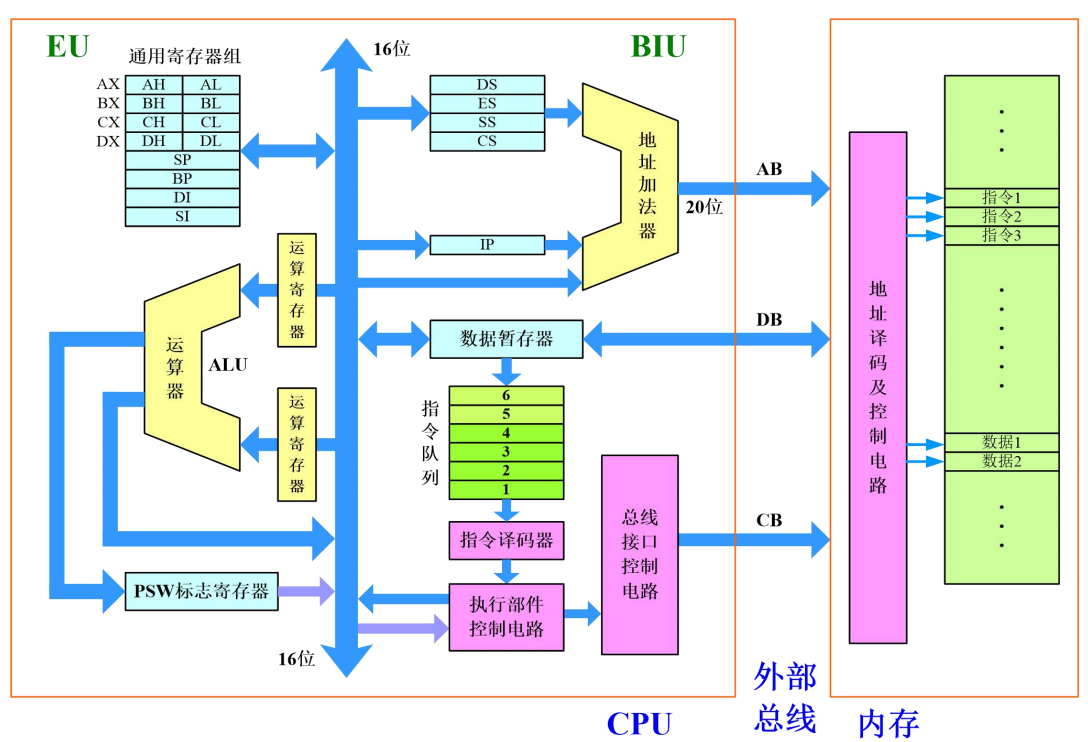
\includegraphics[width = 14cm]{img/2.1-1.png}
    \caption{8086处理器体系结构}
\end{figure}

右侧的BIU是总线接口单元(Bus Interface Unit)负责与存储器、I/O接口传递数据,具体完成:
\begin{enumerate}
    \item 从内存中取指令、送到指令队列
    \item 配合EU从指定的内存单元或I/O端口取数据
    \item 将EU的操作结果送到指定的内存单元或I/O端口
\end{enumerate}

左侧执行单元EU负责指令的执行(算术、逻辑、移位运算,有效地址计算,控制命令、……),包括ALU,通用寄存器组和状态寄存器,进行8/16位运算。


取指令和执行指令在时间上重叠,BIU在指令队列缓冲器有2个以上空字节时就不断从主存连续地址单元中取得指令送入指令队列缓冲器中,EU则不断从指令队列中取出指令译码执行。仅当一下情况发生时,两者并行工作的状态打破:
\begin{enumerate}
    \item 6个字节的指令队列缓冲器满,且EU没有主存或I/O访问请求时,BIU进入空闲状态
    \item EU执行访存或I/O指令时,需要对主存或I/O设备进行读写数据操作,则在BIU执行取指周期后,暂停取指操作,在下一总线执行EU所要求的主存或I/O读写操作,之后再继续BIU的取指操作。
    \item 在EU执行转移、调用、返回等程序跳转指令时,因之前读入指令队列缓冲器的指令已无效,则BIU在清楚缓冲器的同时,根据EU提供的跳转地址,重新获取跳转后的程序指令。
\end{enumerate}


工作原理:

\begin{enumerate}
    \item DB线中取数据到数据暂存器里
    \item 指令队列有2+空字节,则BIU自动取指,放到指令队列中
    \item EU总是从队列前部取指令执行
    \item 指令要访问M或I/O,EU会请求BIU完成
\end{enumerate}

优点:实现了预取指令,取指令和执行指令可以并行,加速程序运行。由于有指令队列,BIU和EU可以并行工作,一边取指令、一边执行指令,构成指令级流水线。

\subsection{寄存器、主存和I/O结构}


\subsubsection{寄存器}

\begin{figure}[H]
    \centering
    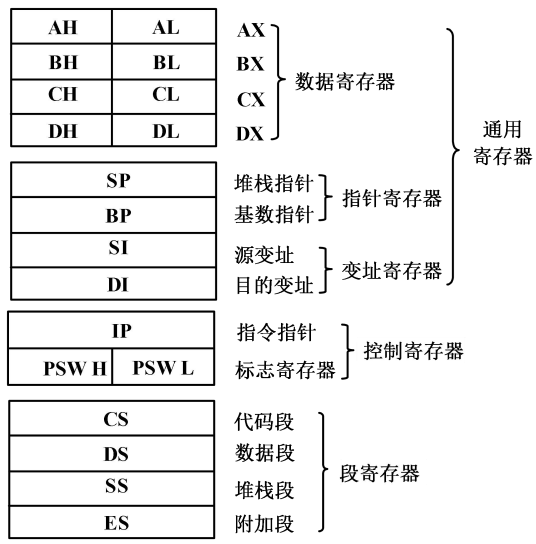
\includegraphics[height=6cm]{img/2.1-2.png}
    \caption{寄存器结构}
\end{figure}

首先是数据寄存器:
\begin{enumerate}
    \item 通用寄存器组均为16位,但是可以拆分成高位和低位转化成8位
    \item AX 用于字乘法、字除法 和 字节乘法、字节除法以及字I/O
    \item BX有时作为 地址寄存器 保存 段内偏移地址 
    \item CX有时作为 隐含计数器 串操作计数 循环计数 CL 移位次数
    \item DX有时作为 地址寄存器 保存 I/O地址
\end{enumerate}

指针寄存器

\begin{enumerate}
    \item SP 堆栈指针寄存器,用于存放主存堆栈区的偏移地址,指示当前操作位置
    \item BP 基数指针寄存器,用于存放主存的基本偏移地址
\end{enumerate}

变址寄存器

\begin{enumerate}
    \item SI 源变址寄存器 指向源操作数
    \item DI 目的变址寄存器 指向目的操作数
    \item SI、DI具有自动修改内容的功能
\end{enumerate}

控制寄存器

\begin{enumerate}
    \item IP 指令指针寄存器,用来指示指令所在存储单元的段内偏移地址。系统将欲执行程序的首地址加载至CS和IP中,转移类指令用跳转的目标地址修改IP(或CS和IP)。当以及CS和IP从主存取指令后IP自动加一,指向下一个读取的指令字节
    \item PSW 是程序状态字,也称为状态寄存器或标志寄存器格式如下
\end{enumerate}

\begin{figure}[H]
    \centering
    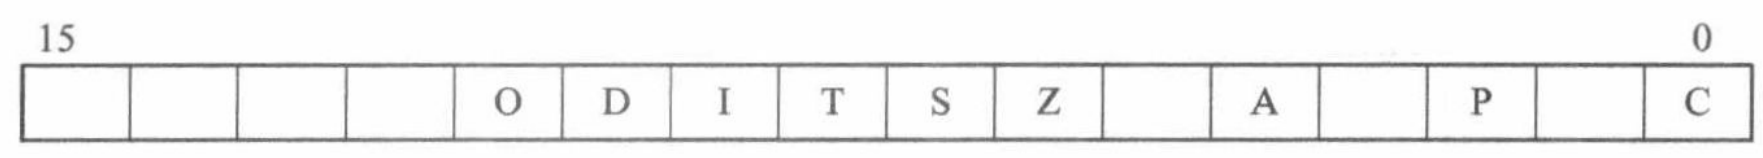
\includegraphics[width=12cm]{img/2.1-3.png}
    \caption{状态标志位的值}
\end{figure}

\begin{enumerate}
    \item  PSW为16位,暂定9个标志位
    \item C——进位标志。加减运算若在最高位出现进位或错位,则标志为1,否则清0.逻辑运算、位移和循环指令也影响该标志位
    \item P——奇偶标志位。低8位中1的个数位偶数时,标志位置位1,否则清0
    \item A——半加进位标志位。加减运算时,低四位向高思维进位或者借位,则置1,否则清0。用于BCD运算结果矫正
    \item Z——零标志位。运算结果全为0,则为1,否则清0
    \item T——陷阱标志位(单步标志位)。为1则进入单步执行指令工作方式,产生单步中断,CPU执行陷阱中断程序。将执行结果显示(寄存器、存储单元和I/O接口)
    \item I——中断允许标志位。为1则可屏蔽中断请求,为0则不可
    \item D——方向标志位。为1则SI和DI在串操作指令执行中自动减即从高到低,否则SI和DI自动增量。
    \item O——溢出标志位。当带符号数运算超出8位或16位表示范围
\end{enumerate}

段寄存器

由于8086的设计,主存是按段划分,分为数据段、堆栈段、代码(程序)段、附加段。

\begin{enumerate}
    \item 代码段寄存器CS  指示程序区
    \item 数据段寄存器DS 指示数据区
    \item 堆栈段寄存器SS 指示堆栈区
    \item 附加段寄存器ES 指示数据区
\end{enumerate}

\begin{enumerate}
    \item SS:SP $\rightarrow$ 堆栈地址
    \item CS:IP $\rightarrow$ 主存地址 类似PC
    \item 首先找段地址寄存器+段内偏移地址
    \item 地址加法器只做地址加法,输出为I/O、存储器地址
\end{enumerate}



\newpage

\subsubsection{主存结构}

双体结构,既可以实现16位存储,也可以实现8位存储

\begin{figure}[H]
    \centering
    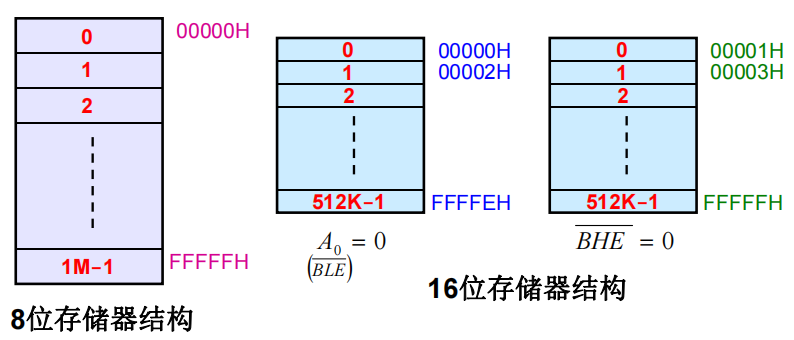
\includegraphics[height=4cm]{img/2.1-4.png}
    \caption{双体结构}
\end{figure}

分段结构

\begin{enumerate}
    \item 代码、数据量不大->使其处于同一段内(64KB范围内)->减少指令长度、提高运行速度
    \item 内存分段为程序的浮动分配创造条件
    \item 形成地址6832H:1280H->物理地址 = 68320H+1280
    \item 各个分段之间可以重叠
    
    \begin{figure}[H]
        \centering
        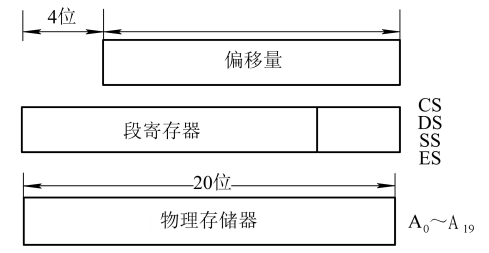
\includegraphics[height=4cm]{img/2.1-5.png}
        \caption{物理地址形成}
    \end{figure}
\end{enumerate}


\begin{figure}[H]
    \centering
    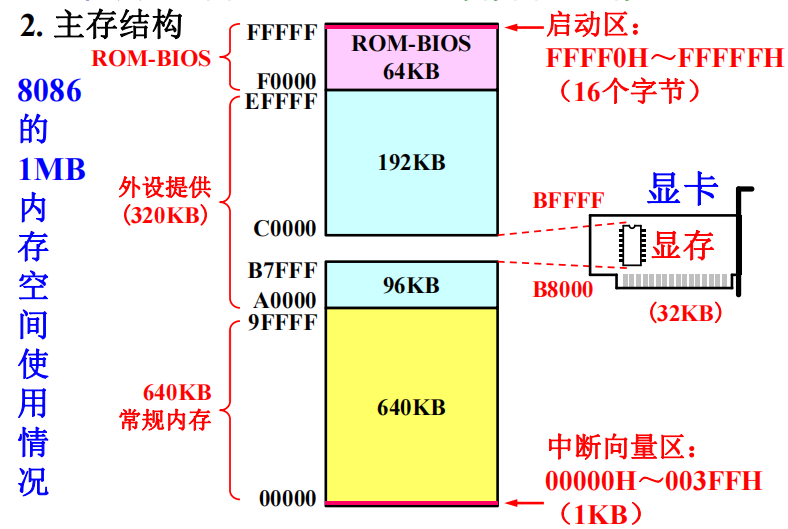
\includegraphics[height=6cm]{img/2.1-7.png}
    \caption{主存结构}
\end{figure}

\subsubsection{I/O地址空间}

BIU处的地址加法器,将16位段地址左移4位,然后与16位段内偏移地址相加,生成20位物理地址,即
\begin{equation}
    \text{物理地址}=\text{段地址}\times 16 + \text{段内偏移地址}
\end{equation}

其中:段地址由16位段寄存器提供,段内偏移地址由IP或EU确定的有效地址EA提供

8086处理器提供20位地址,对主存单元寻址时使用全部20位地址,对I/O设备端口寻址使用其低16位地址,使主存有1M的存储空间,I/O设备有64k的端口空间(两个字节)

8086采用字节编制,即主存或I/O的一个地址单元内存储一个字节,拥有一个字节编号,使得处理器可以根据地址进行1字节的存储器或I/O设备的读写操作

\begin{figure}[H]
    \centering
    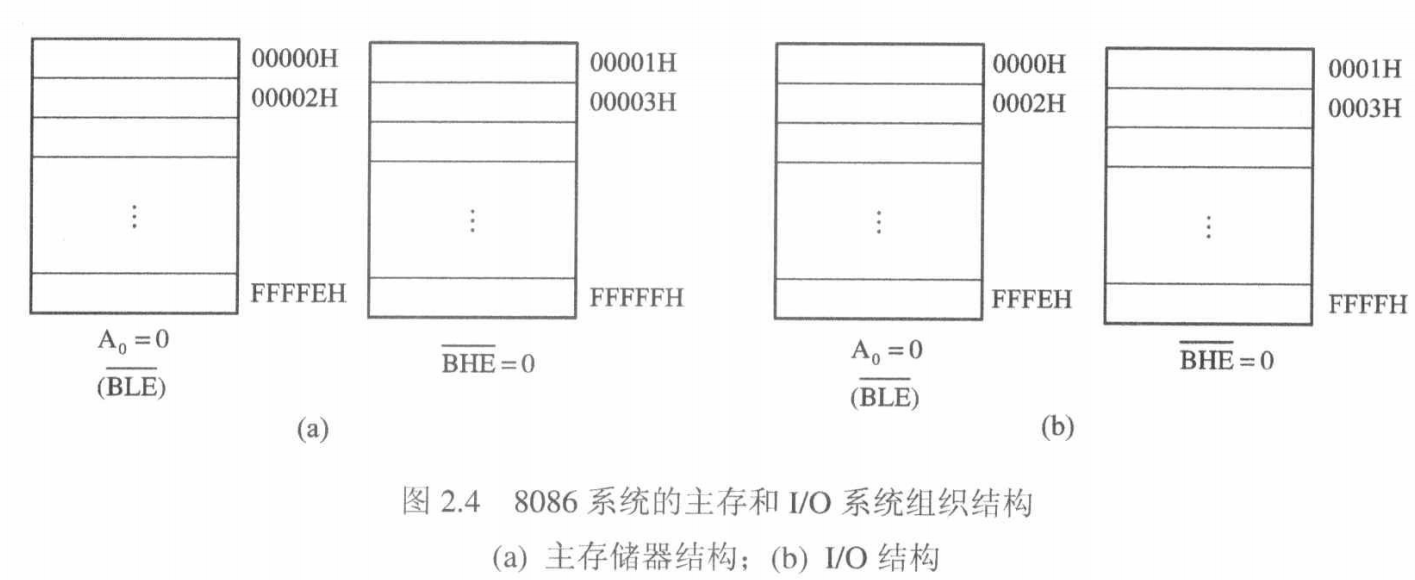
\includegraphics[width=10cm]{img/2.2-1.png}
\end{figure}

主存与I/O地址空间均按地址的奇偶分为两个体,偶地址空间对应低字节,8086使用低字节允许信号$A_0=0$选择;奇地址空间对应高字节的访问用高字节允许信号$\overline{BHE}=0$选择,具体选择如下:

\begin{figure}[H]
    \centering
    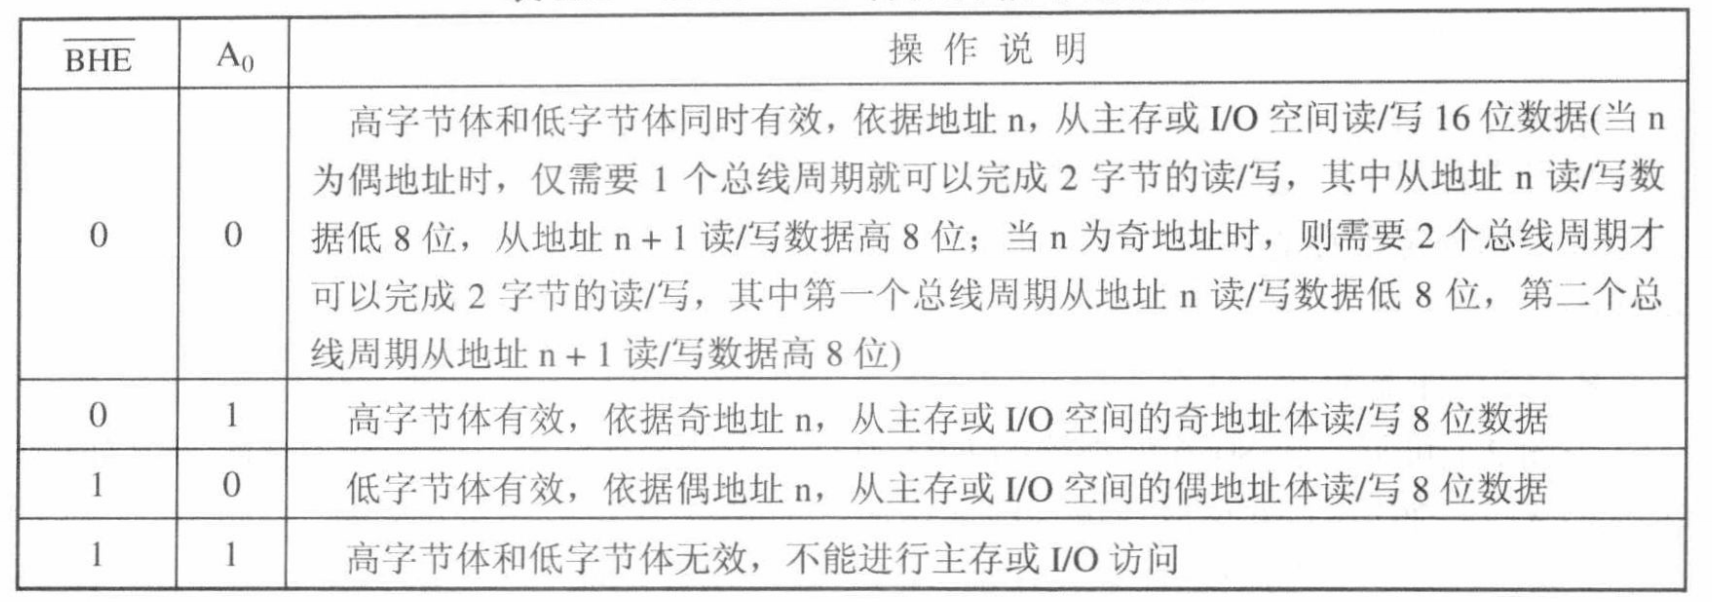
\includegraphics[width=12cm]{img/2.2-2.png}
    \caption{8086 CPU 允许信号的作用}
\end{figure}

8086将1MB存储空间分为若干个存储段,每段固定64KB大小,用16位段地址寻址,每段的起始地址位xxxx0000,低四位为0。且由于段地址由16位段寄存器提供,所以1MB可以划分$2^{16}$个重叠段,不重叠有$2^{4}$个

分段结构使16位地址的寻址空间64KB扩大到1MB,设置了4个属性的存储段:代码段、数据段、堆栈段和附加段。段寄存器CS,DS,SS和ES分别为4个属性段提供段地址。

\begin{enumerate}
    \item 程序段存放指令代码
    \item 数据段存放原始数据、中间结果和最终结果
    \item 堆栈段用来设立堆栈
    \item 好处是减少程序数据和堆栈的冲突
\end{enumerate}

\begin{figure}[H]
    \centering
    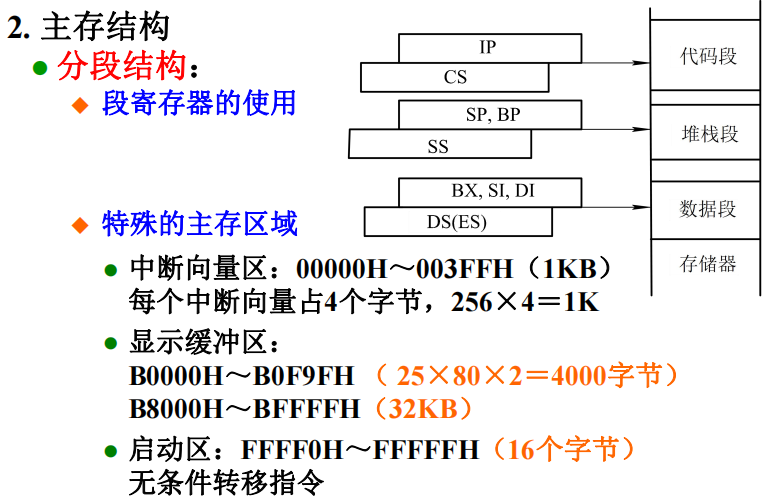
\includegraphics[height=6cm]{img/2.1-6.png}
    \caption{分段结构}
\end{figure}

各类的访存操作中,段地址由默认或指定的段寄存器提供,CPU根据指令中提供的段内偏移地址来源自动的默认使用段寄存器。

段寄存器DS、SS和ES的内容用传送指令加载,但是任何传送指令不能向代码段寄存器CS加载。JMP CALL RET INT IRET等可以设置和影响CS。无论程序去、数据区还是堆栈区都可以超过64KB的容量,都可以利用重新设置段寄存器内容的方法加以扩大


\begin{enumerate}
    \item I/O地址空间独立于主存地址空间,两者采用不同的读写信号进行访问控制
    \item I/O地址空间包含64k个可单独寻址的8位I/O端口,编号0到FFFFH,其中I/O端口地址0F8H~0FFH被保留
    \item 16位系统I/O也按地址的奇偶分为个体
\end{enumerate}
\begin{figure}[H]
    \centering
    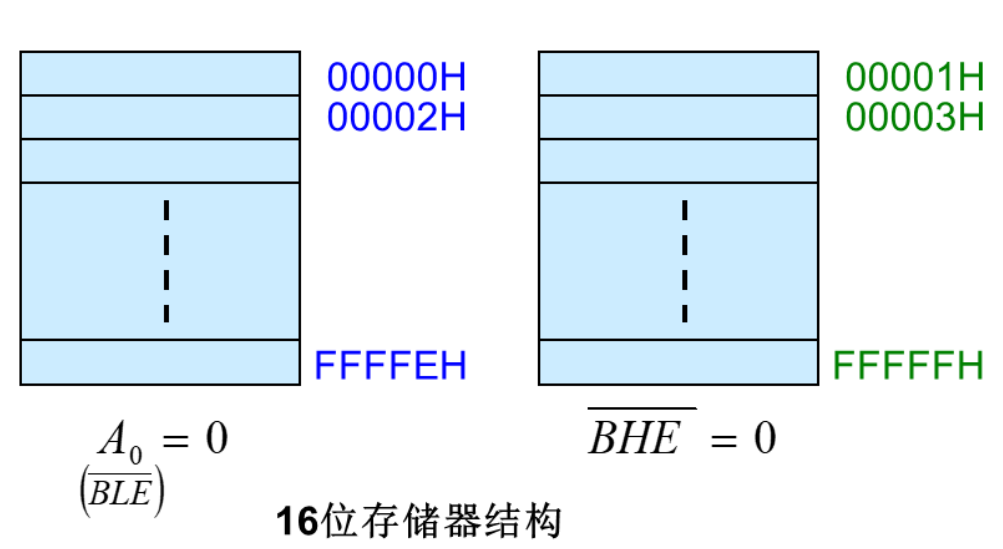
\includegraphics[height=6cm]{img/2.1-8.png}
    \caption{I/O结构}
\end{figure}

\subsubsection{处理器芯片引脚}

\begin{figure}[H]
    \centering
    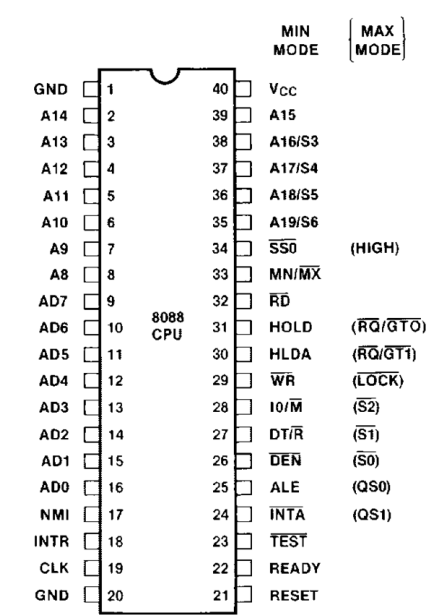
\includegraphics[height=10cm]{img/2.1-9.png}
    \caption{8086引脚图}
\end{figure}

8086与8088对比:
\begin{enumerate}
    \item 内部指令预期队列6字节→4字节
    \item 8088:AD7~AD0 8086 AD15~AD0(速度快)
    \item 8088 $\bar{SS0}$ 8086 $\bar{BHE}$/S7
    \item 8088 I/O/$\bar{M}$ 8086 $\bar{M}$/I/O
\end{enumerate}

引脚$MN/\overline{MX}=1$时,8086工作在最小模式,微机中只有一个处理器。而当$MN/\overline{MX}=0$时,允许接入其他协处理器(运算处理器8087 I/O处理器8089),此时系统总线有8086和总线控制器8288提供的信号共同形成,以支持多微处理器系统构成。

两种模式下的共用信号

\begin{enumerate}
    \item  $A_{16}\sim A_{19}/S_3\sim S_6$(输出,三态):高4位地址$A_{16}\sim A_{19}$与状态$S_3\sim S_6$分时复用信号。状态$S_6$始终为低。$S_5$表示中断允许标志,在每个时钟周期开始时被更新。$S_4$和$S_3$用来指示CPU正在使用的段寄存器,其编码状态如下表。而高4位地址$A_{16}\sim A_{19}$在CPU访问I/O时输出低电平,在一些特殊情况下还可以处于高阻状态。
\begin{table}[H]
    \centering
    \begin{tabular}[]{ccc}
        \hline
        $S_4$ & $S_3$ & 指示的寄存器 \\
        \hline
        0 & 0 & ES\\
        0 & 1 & SS\\
        1 & 0 & CS或不用\\
        1 & 1 & DS \\
        \hline
    \end{tabular}
\end{table}

\item  $AD_0 \sim  AD_{15}$(输入输出、三态):地址$A_0 \sim A_{15}$与数据$D_0 \sim D_{15}$分时复用信号。 CPU读写主存或者I/O设备时,在总线周期的$T_1$时钟周期,地址信号有效,之后允许数据或状态信号有效。

\item  $\overline{BHE}/S_7$(输入输出、三态): 高字节允许与状态$S_7$分时复用信号。在总线周期的$T_1$时钟周期$\overline{BHE}$起作用。$S_7$为备用状态。

\item  RESET(输入):复位信号,高电平有效,复位脉冲至少持续4个时钟周期。RESET返回低电平时,CPU重新启动。CPU内部状态如下:

\begin{figure}[H]
    \centering
    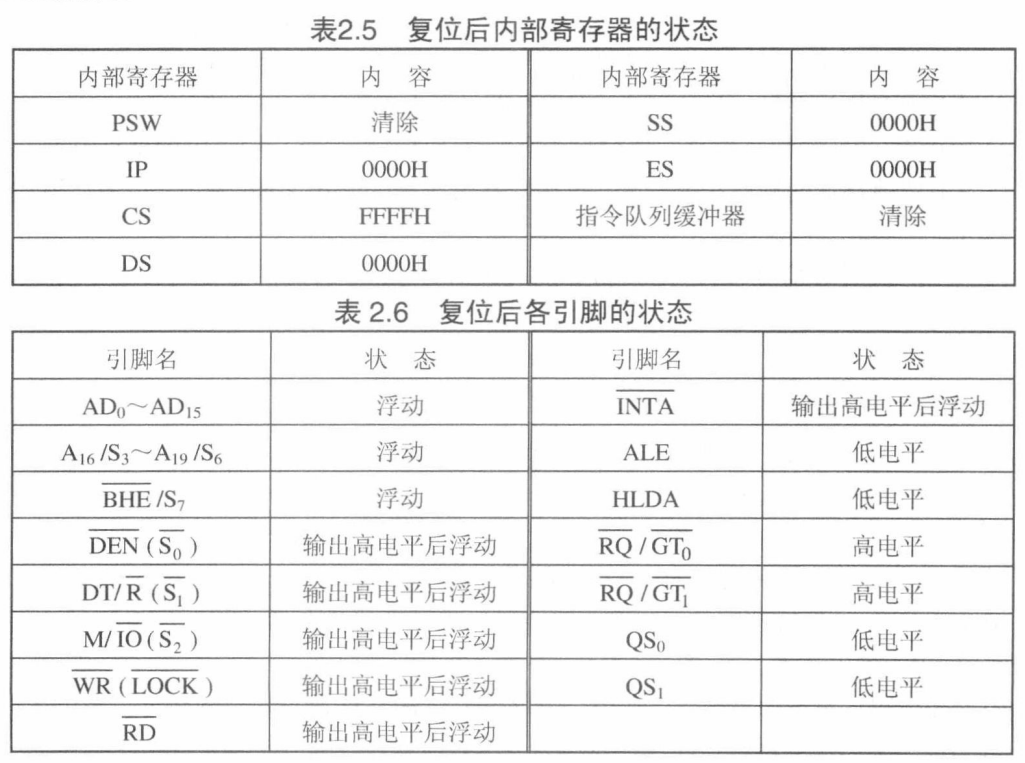
\includegraphics[width=12cm]{img/2.2-4.png}
\end{figure}

\item  READY(输入):准备就绪信号,高电平有效。CPU读写内存或I/O设备时,在总线周期$T_3$时钟周期采样READY信号。若为高,则表示设备已经准备好,若为低电平,则表示被访问的存储器或设备没有完成读写,需要插入等待周期$T_{WAIT}$,在等待周期继续采样READY信号,直至READY变为有效(高电平),进入$T_4$周期,完成数据读写。

\item  $\overline{TEST}$(输入):测试信号,低电平,用于与其他处理器(8087)同步执行程序。CPU执行WAIT指令时测试该引脚,当该信号无效时,CPU进入等待状态(空转);一旦该信号有效,CPU退出等待,继续执行程序。这个信号在每个时钟周期的上升沿由内部电路进行同步。

\item INTR(输入):可屏蔽中断请求信号,高电平有效。CPU在每条指令执行的最后一个时钟周期采样该信号,以决定是否进入中断响应(INTA)周期。用软件复位中断允许标志(IF=0),可以屏蔽该中断请求。

\item NMI(输入):非屏蔽中断请求信号,上升沿有效。该请求信号不可被屏蔽,中断一定会发生。NMI>INTR

\item $\overline{INTA}$(输出、三态):对INTR中断请求的响应信号。在响应中断过程中,由$\overline{INTA}$送出两个负脉冲(两个INTA周期),在第二个INTA周期CPU获得外部中断源的中断向量码。最小模式由8086提供,最大模式时由8288提供。

\item $DT/\overline{R}$(输出、三态):数据发送/接收控制信号,用于确定数据的传送方向。高电平控制数据发送,即CPU将数据写到主存或I/O接口;低电平控制数据接收,从主存或I/O接口读取数据。用于数据总线驱动器8286/8287或74245的方向控制。该信号在最小模式时用8086提供,在最大模式时用8288提供。

\item $\overline{DEN}$(输出、三态):数据有效信号。该信号有效时,表示$D_0 \sim D_{15}$上的数据有效。该信号在最小模式时由8086提供,最大模式时由8288提供。

\end{enumerate}
仅在最小模式下使用的信号




\end{document}